% Created 2024-10-16 śro 21:35
% Intended LaTeX compiler: pdflatex
\documentclass[../main.tex]{subfiles}

% \usepackage[a4paper, margin=3cm]{geometry}
% \usepackage{amssymb} // not working

\usepackage[T1]{fontenc}
\usepackage[utf8]{inputenc}
\usepackage{graphicx}
\usepackage{longtable}
\usepackage{wrapfig}
\usepackage{rotating}
\usepackage[normalem]{ulem}
\usepackage{amsmath}
\usepackage{capt-of}
\usepackage{hyperref}
\usepackage{siunitx}
\usepackage{float}
\usepackage[polish]{babel}

\graphicspath{{../}}
\author{Wojciech Paderewski}
\date{\today}
\title{Koncepcja ukladu}
\hypersetup{
 pdfauthor={Wojciech Paderewski},
 pdftitle={Koncepcja ukladu},
 pdfkeywords={},
 pdfsubject={},
 pdflang={Polish}}

\begin{document}

\section{Koncepcja układu}
Koncepcją układu jest zaprojektowanie i wykonanie budzika opartego o lampy Nixie, który będzie synchronizował się dzięki odpytywaniu serwera NTP oraz
z wykorzystaniem modułu RTC wbudowanego w mikrokontroler.

\subsection{Założenia projektowe}
\begin{itemize}
    \item Funkcjonalność ustawiania godziny budzika bedzie realizowana przez zewnętrzny serwer dla wygody użytkownika, który nie musi dostosowywać czasu ręcznie.
    \item Na wyświetlaczu Nixie będą wyświetlane godziny, minuty, sekundy.
    \item Od spodu obudowy będą umieszczone paski LED, które będą podświetlały obudowę i będzie można ustawić na nich animacje podczas alarmu.
    \item Alarm będzie sygnalizowany dźwiękiem oraz miganiem pasków LED.
    \item Dźwięk może być grany z głośnika wbudowanego w obudowę lub z zewnętrznego głośnika komunikującego się z serwerem przez Wi-Fi.
    \item Wyłączanie alarmu będzie możliwe poprzez przycisk na obudowie, aplikację mobilną lub zewnętrzny przycisk połączony z serwerem.
    \item W przypadku braku połączenia z serwerem, czas będzie mierzony przez RTC wbudowany w mikrokontroler.
    \item Programowa oraz manualna regulacja jasności wyświetlacza Nixie oraz pasków LED.
\end{itemize}

Powyższe założenia projektowe będą skutkować bardzo wszechstronnym budzikiem, który będzie miał wyglad retro,
ale z nowoczesnymi funkcjonalnościami.

\subsection{Wstępne obliczenia i założenia}

Pierwszą rzeczą, która została wykonana to zakup lamp Nixie, które będą wykorzystane w projekcie. 
Przez coraz bardziej ograniczony dostęp do tych lamp, 
zdecydowano się na zakup lamp Z570M, które zostały zakupione w ilości 6 sztuk. Lampy te mają 10 cyfr oraz kropkę dziesiętną,
która nie jest nam potrzebna, ale została przewidziana możliwość jej sterowania w razie potencjalnego zastosowania w przyszłości.

Kluczowe parametry zastosowanych lamp nixie odczytane z noty katalogowej:
\begin{itemize}
    \item Napięcie zapłonu: \SI{170}{\volt}
    \item Napięcie wygaszania: \SI{120}{\volt}
    \item Napięcie pracy: \SI{150}{\volt}
    \item Prąd katodowy średni: \SI{2}{\milli\ampere}
\end{itemize}

W celu zweryfikowania działania lamp nixie i sprawdzenia parametrów zasilania, został wykonany prototyp układu z jedną lampą nixie,
wykorzystujący zasilacz impulsowy HV z regulowanym napięciem wyjściowym zakupiony w sklepie internetowym.

Zakupiona przetwornica HV ma następujące parametry:
\begin{itemize}
    \item Napięcie wejściowe: \SI{5}-\SI{12}{\volt}
    \item Napięcie wyjściowe: \SI{150}-\SI{220}{\volt}
    \item Prąd wyjściowy: \SI{20}{\milli\ampere}
\end{itemize}

W celu sprawdzenia działania lampy musimy najpierw dobrać rezystor ograniczający prąd katodowy.
Zakładając, że napięcie zasilania wynosi maksymalnie $U_{\text{max}} = \SI{220}{\volt}$, a napięcie zapłonu lampy $U_{\text{zap}} = \SI{170}{\volt}$,
przy prądzie katodowym $I_{\text{kat}} = \SI{2}{\milli\ampere}$, rezystor ograniczający prąd katodowy można obliczyć ze wzoru:

\begin{equation}
    R = \frac{U_{\text{max}} - U_{\text{zap}}}{I_{\text{kat}}} = \frac{\SI{220}{\volt} - \SI{150}{\volt}}{\SI{2}{\milli\ampere}} = \SI{35}{\kilo\ohm}
\end{equation}

W nocie katalogowej lampy nixie Z570M producent podaje, że zalecany rezystor ograniczający prąd katodowy 
powinien mieć wartość \SI{33}{\kilo\ohm} dla napięcie zasilania \SI{200}{\volt}, więc wartość \SI{35}{\kilo\ohm} dla napięcia \SI{220}{\volt}
wydaje się obliczona prawidłowo, taki też rezystor ma zostać użyty w faktycznym układzie.

Zatem rezystor ograniczający prąd katodowy powinien mieć wartość około \SI{35}{\kilo\ohm}.
Do testu użyto rezystora o wartości \SI{22}{\kilo\ohm} oraz rezystora o wartości \SI{10}{\kilo\ohm}, połączonych
szeregowo, co daje wartość \SI{32}{\kilo\ohm}, co jest wartością zbliżoną do obliczonej.

\begin{figure}[H]
    \centering
    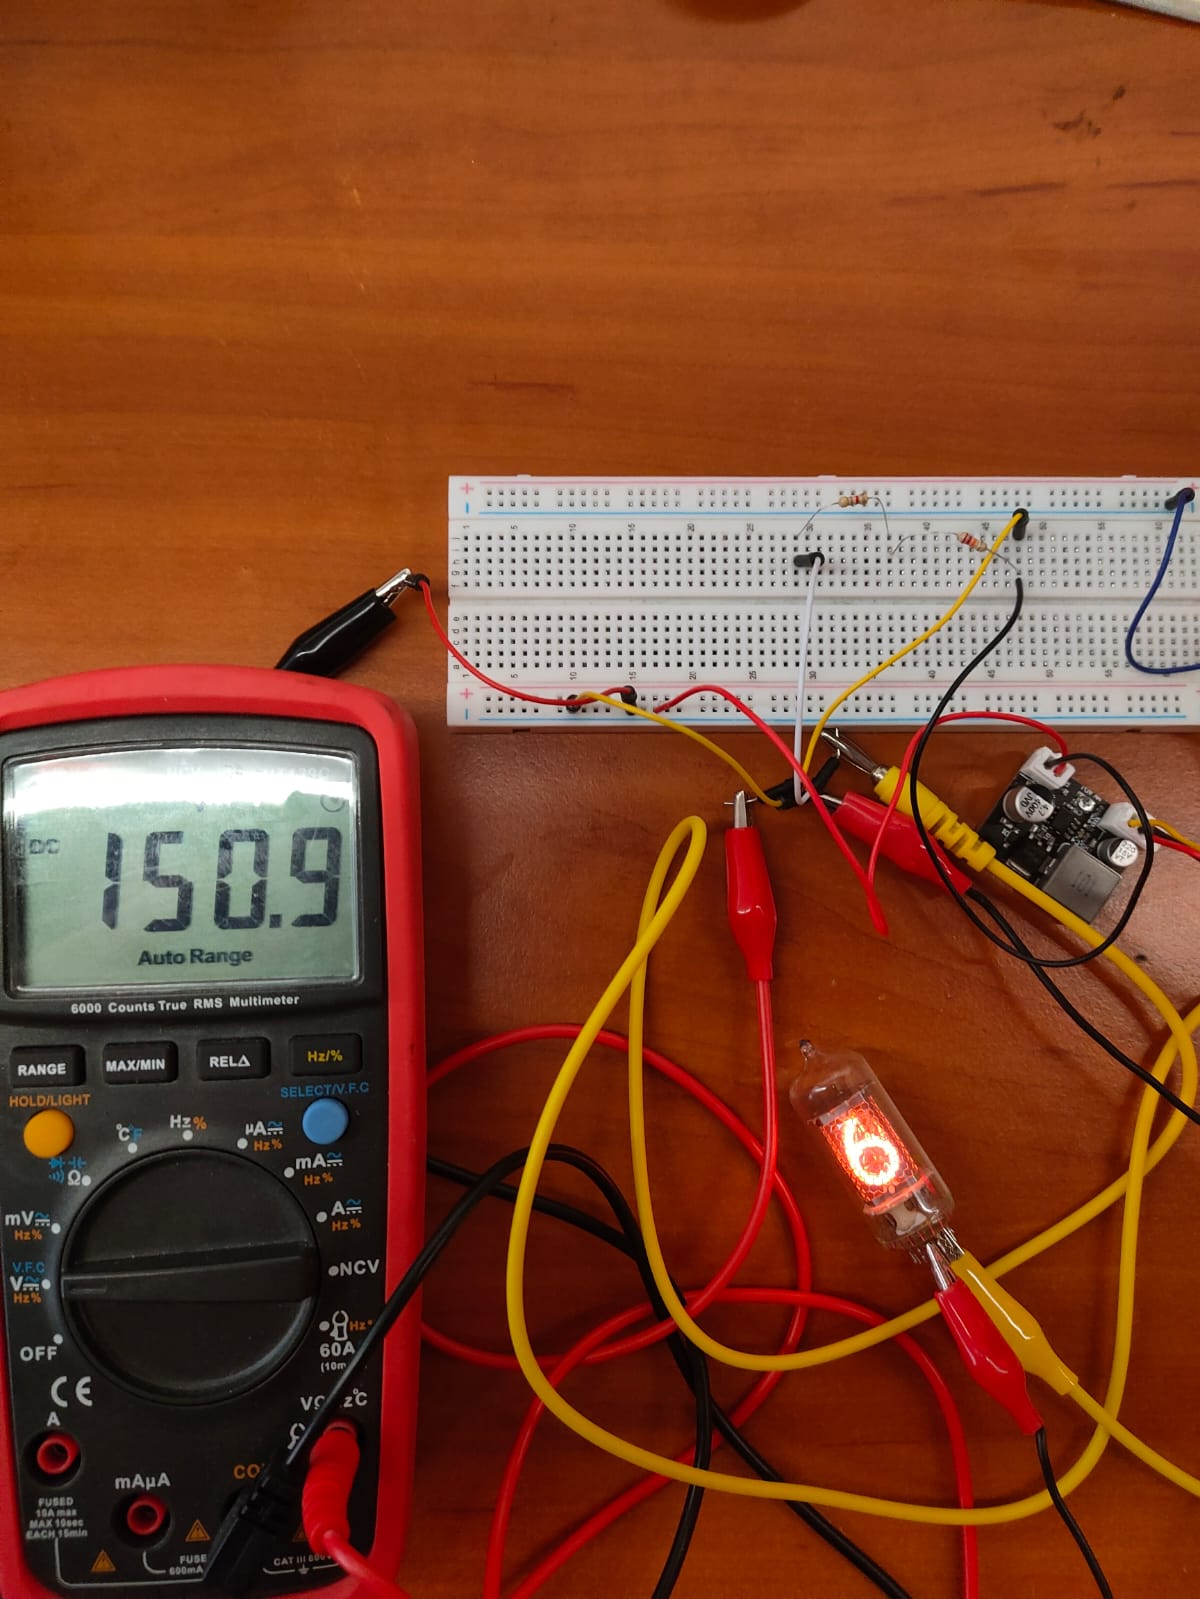
\includegraphics[width=0.5\textwidth]{nixie150V.jpeg}
    \caption{Prototyp układu z lampą nixie przy napięciu zasilania \SI{150}{\volt}}
\end{figure}

\begin{figure}[H]
    \centering
    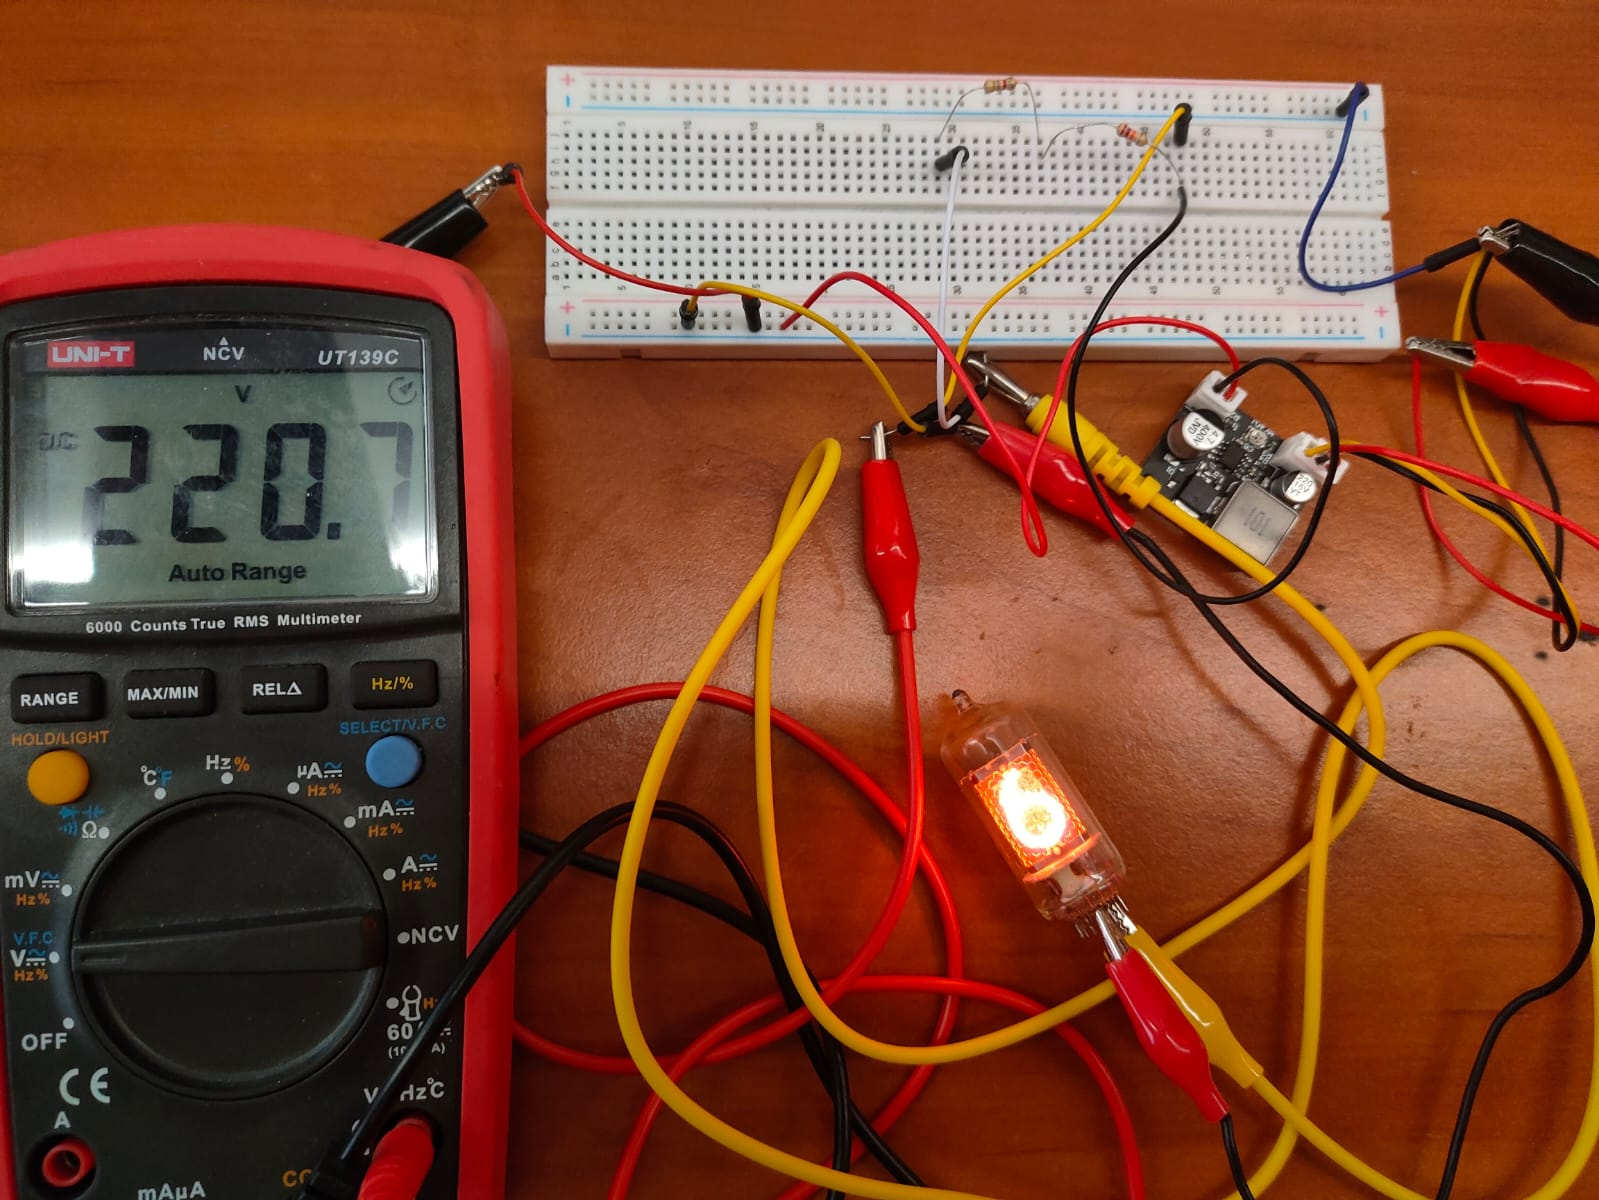
\includegraphics[width=0.5\textwidth]{nixie220V.jpeg}
    \caption{Prototyp układu z lampą nixie przy napięciu zasilania \SI{220}{\volt}}
\end{figure}

Z testów wynika, że lampy nixie działają poprawnie, a dobrany rezystor ograniczający prąd katodowy jest odpowiedni. 
Przy napięciu zasilania \SI{150}{\volt} lampa świeci słabiej, ale jest to zgodne z oczekiwaniami,
natomiast przy napięciu \SI{220}{\volt} lampa świeci jasno i pojawiają się lekko niebieskie refleksy wewnątrz lampy, co jest zgodne z oczekiwaniami.

Nie sprawdzono napięcia wygaszania, ponieważ zasilacz nie pozwalał na takie napięcie, 
ale ustalono, że lampa nawet przy napięciu \SI{150}{\volt} była w stanie zapłonąć i świecić poprawnie.

Z testów można wyciągnąć następujące wnioski:

\begin{itemize}
    \item Lampy nixie działają poprawnie przy napięciu zasilania \SI{150}{\volt} oraz \SI{220}{\volt}.
    \item Dobrany rezystor ograniczający prąd katodowy jest odpowiedni.
    \item Lampa nixie Z570M jest w stanie zapłonąć i świecić przy napięciu wygaszania \SI{150}{\volt}.
    \item Zakres regulacji napięcia na zasilaczu HV powinien być większy np. \SI{130}-\SI{250}{\volt}, by lampa mogła być jeszcze słabiej podświetlona, może się to okazać przydatne w nocy.
\end{itemize}

\subsection{Dobór mikrokontrolera}

Następnie wybrano mikrokontroler, który będzie użyty w projekcie. Wybrano mikrokontroler ESP32-S3, który jest nowym mikrokontrolerem z wbudowanym modułem Wi-Fi oraz Bluetooth.
Mikrokontroler ten ma wbudowany programator co pozwoli na łatwe wgrywanie oprogramowania, bez zewnętrznego programatora, a także ma wbudowany moduł RTC,
co pozwoli na zachowanie czasu, pomiędzy zapytaniami do serwera NTP.

Wybrany układ ma również wystarczająco dużo pinów GPIO, by móc obsłużyć wszystkie lampy nixie, paski LED, głośnik oraz przyciski.
Posiada on układ dwu rdzeniowy, co w razie potrzeby pozwoli na obsługę wielowątkowości. Zegar procesora ma częstotliwość \SI{240}{\mega\hertz},
co w zupełności wystarczy do obsługi wszystkich elementów układu.

\subsection{Dobór paska LED}
Do budzika wybrano adresowalne paski LED WS2812B, 
które są bardzo popularne w projektach DIY, ponieważ są łatwe w obsłudze, mają wbudowany kontroler,
który pozwala na sterowanie każdym diodą z osobna oraz są dostępne w różnych długościach i kolorach.
Wybrano pasek z diodami RGB, co pozwoli na wyświetlanie wielu kolorów. Moc na metr wynosi \SI{18}{\watt}.
Pasek posiada też stopień ochrony IP65, czyli powinien być odporny na kurz oraz wilgoć.

\subsection{Koncepcja zasilania}
Projekt sekcji zasilania został rozpoczęty od oszacowania mocy potrzebnej do zasilania całego układu.
Poza lampami nixie, najbardziej obciążającym elementem będzie pasek LED oraz mikrokontroler, pozostałe elementy będą pobierały znikome ilości prądu.

Założono maksymalną długość paska LED na \SI{30}{\centi\meter}. Z deklaracji producenta paska LED wynika, że moc na metr wynosi \SI{18}{\watt}, co daje:
\begin{equation}
    P_{\text{LED}} = \SI{18}{\watt\per\meter} \cdot \SI{0.3}{\meter} = \SI{5.4}{\watt}
\end{equation}
Następnie obliczono prąd potrzebny do zasilenia paska LED przy napięciu \SI{5}{\volt}:
\begin{equation}
    I_{\text{LED}} = \frac{P_{\text{LED}}}{U_{\text{LED}}} = \frac{\SI{5.4}{\watt}}{\SI{5}{\volt}} = \SI{1.08}{\ampere}
\end{equation}

Następnie obliczono moc potrzebną do zasilania mikrokontrolera ESP32-S3, według producenta maksymalny pobór prądu wynosi \SI{340}{\milli\ampere},
co przy napięciu zasilania \SI{3.3}{\volt} daje:

\begin{equation}
    P_{\text{ESP32}} = \SI{340}{\milli\ampere} \cdot \SI{3.3}{\volt} = \SI{1.122}{\watt}
\end{equation}

Następnie policzono prąd pobierany przez wszystkie lampy, których jest 6 sztuk, przy prądzie katodowym \SI{2}{\milli\ampere} każda, co daje:
\begin{equation}
    I_{\text{Nixie}} = 6 \cdot \SI{2}{\milli\ampere} = \SI{12}{\milli\ampere}
\end{equation}

Następnie obliczono moc potrzebną do zasilania lampy nixie, przy napięciu \SI{220}{\volt} oraz prądzie wszystkich lamp \SI{12}{\milli\ampere}, zakładając 
sprawność przetwornicy na poziomie \SI{70}{\percent}:

\begin{equation}
    P_{\text{Nixie}} = \frac{U_{\text{Nixie}} \cdot I_{\text{Nixie}}}{\text{Sprawność}} = \frac{\SI{220}{\volt} \cdot \SI{12}{\milli\ampere}}{\SI{0.7}{}} = \SI{3.43}{\watt}
\end{equation}

Pozostałe komponenty będą pobierały znikome ilości prądu, więc nie będą brane pod uwagę w obliczeniach.
Szacunkowa moc potrzebna do zasilania całego układu wynosi:

\begin{equation}
    P_{\text{całkowita}} = P_{\text{LED}} + P_{\text{ESP32}} + P_{\text{Nixie}} = \SI{5.4}{\watt} + \SI{1.122}{\watt} + \SI{3.43}{\watt} = \SI{9.952}{\watt}
\end{equation}

Szacunkowa moc potrzebna do zasilania całego układu wynosi około \SI{10}{\watt}, co powoduje problem z zasilaniem z gniazd USB w komputerze,
ponieważ maksymalna moc, jaką można pobrać z gniazda USB wynosi \SI{2.5}{\watt}, co jest zdecydowanie za mało.

Problem jest też projekt przetwornicy HV zasilanej z 5V, ponieważ przetwornica boost przy takiej aplikacji miała by bardzo wysokie wypełnienie rzędu 95 \%,
co prowadziło by do dużych start mocy.

Alternatywą jest przetwornica flyback, która ma mniejsze wypełnienie i była by bardziej wydajna, ale jest bardziej skomplikowana w projektowaniu i montażu.
Podczas prób projektowania takiej przetwornicy, problem okazało się znaleźć odpowiedni transformator, który miał by odpowiednie parametry,
a także byłby dostępny w sklepach elektronicznych.

W związku z tymi problemami, zdecydowano się na zasilanie z zewnętrznego zasilacza 12V, który będzie zasilany z gniazda sieciowego, 
podłączonego do budzika za pomocą złącza DC-Plug. Do programowania mikrokontrolera będzie służyć złącze USB-C.

Ostatecznie sekcja zasilania została podzielona na kilka podsekcji:
\begin{itemize}
    \item Przetwornica 12V na 5V do zasilania pasków LED.
    \item Regulowana przetwornica 12V na HV do zasilania lamp nixie.
    \item LDO 5V na 3.3V do zasilania mikrokontrolera.
\end{itemize}

\subsection{Koncepcja sterowania lampami nixie}
Kolejnym krokiem było zaprojektowanie sekcji sterowania lampami nixie, która będzie odpowiedzialna za wyświetlanie odpowiednich cyfr na lampach.
Jest kilka sposobów na sterowanie lampami:

\begin{itemize}
    \item Sterowanie bezpośrednie - każda lampa ma swoje wejście i jest sterowana osobno za pomocą tranzystora HV połączonego z mikrokontrolerem.
    Niestety wymagane jest wiele pinów GPIO również trzeba użyć ponad 60 tranzystorów HV, co jest bardzo kosztowne.
    \item Multiplexing - wszystkie lampy są podłączone do jednego drivera, który wybiera katode i załączamy odpowiednią anodę. 
    Wymaga to mniej pinów GPIO bo tylko 10, ale multipleksacja powoduje szybsze zużycie lamp i pojawia się efekt migotania(ghosting).
    \item Wykorzystanie dedykowanych driverów - istnieją specjalne układy scalone, które są przeznaczone do sterowania lampami nixie, niestety
    one również wymagają wielu pinów GPIO po 4 na każdą lampę, co daje 24 wymaganych pinów GPIO.
    \item Rejestr przesuwny HV - najbardziej optymalne rozwiązanie, wymaga tylko 3 pinów GPIO. Rejestry HV są ciężko dostępne i dość drogie,
    wymagane jest też by były to rejestry z zatrzaskiem, aby uniknąć efektu ghostingu.
\end{itemize}

W projekcie zdecydowano się na wykorzystanie rejestrów przesuwnych HV. Znaleziono 32 kanałowy rejestr 
HV5530PG-G firmy Microchip mogące pracować z napięciem do \SI{300}{\volt} oraz posiadające zatrzask i wyjście Open Drain.

Rodzaj wyjścia open drain jest bardzo istotny, ponieważ na wyjściu znajduje się stan wysokiej impedancji, co nie powoduje zwierania wszystkich wyjść do masy.
W przypadku wyjścia push-pull, stan wysoki jak i niski powodował by zapalenie się wszystkich lamp, ponieważ spadek napięcia na lampach
nawet w stanie wysokim byłby na tyle duży, że lampy były by w stanie zapłonąć.

Do sterowania 6 lampami potrzebne są 2 rejestry HV5530PG-G, co daje 64 kanały, co pozwoli na sterowanie 6 lampami nixie oraz 2 neonówkami, które
służą jako separator między godzinami, minutami i sekundami. Do sterowania kropkami dziesiętnymi, wykorzystano tranzystory HV połączone z mikrokontrolerem.

Sterowanie lampami z wykorzystaniem rejestru jest proste, wymaga wgrania do rejestru 64 bitów, które odpowiadają za stan lamp oraz przełączanie
zatrzasku co sekundę, aby zmienić ich stan.

\newpage

\subsection{Schemat blokowy układu}
Na rysunku \ref{fig:schemat_blokowy} przedstawiono schemat blokowy układu, który pokazuje jak poszczególne sekcje układu są ze sobą połączone.

\begin{figure}[H]
    \centering
    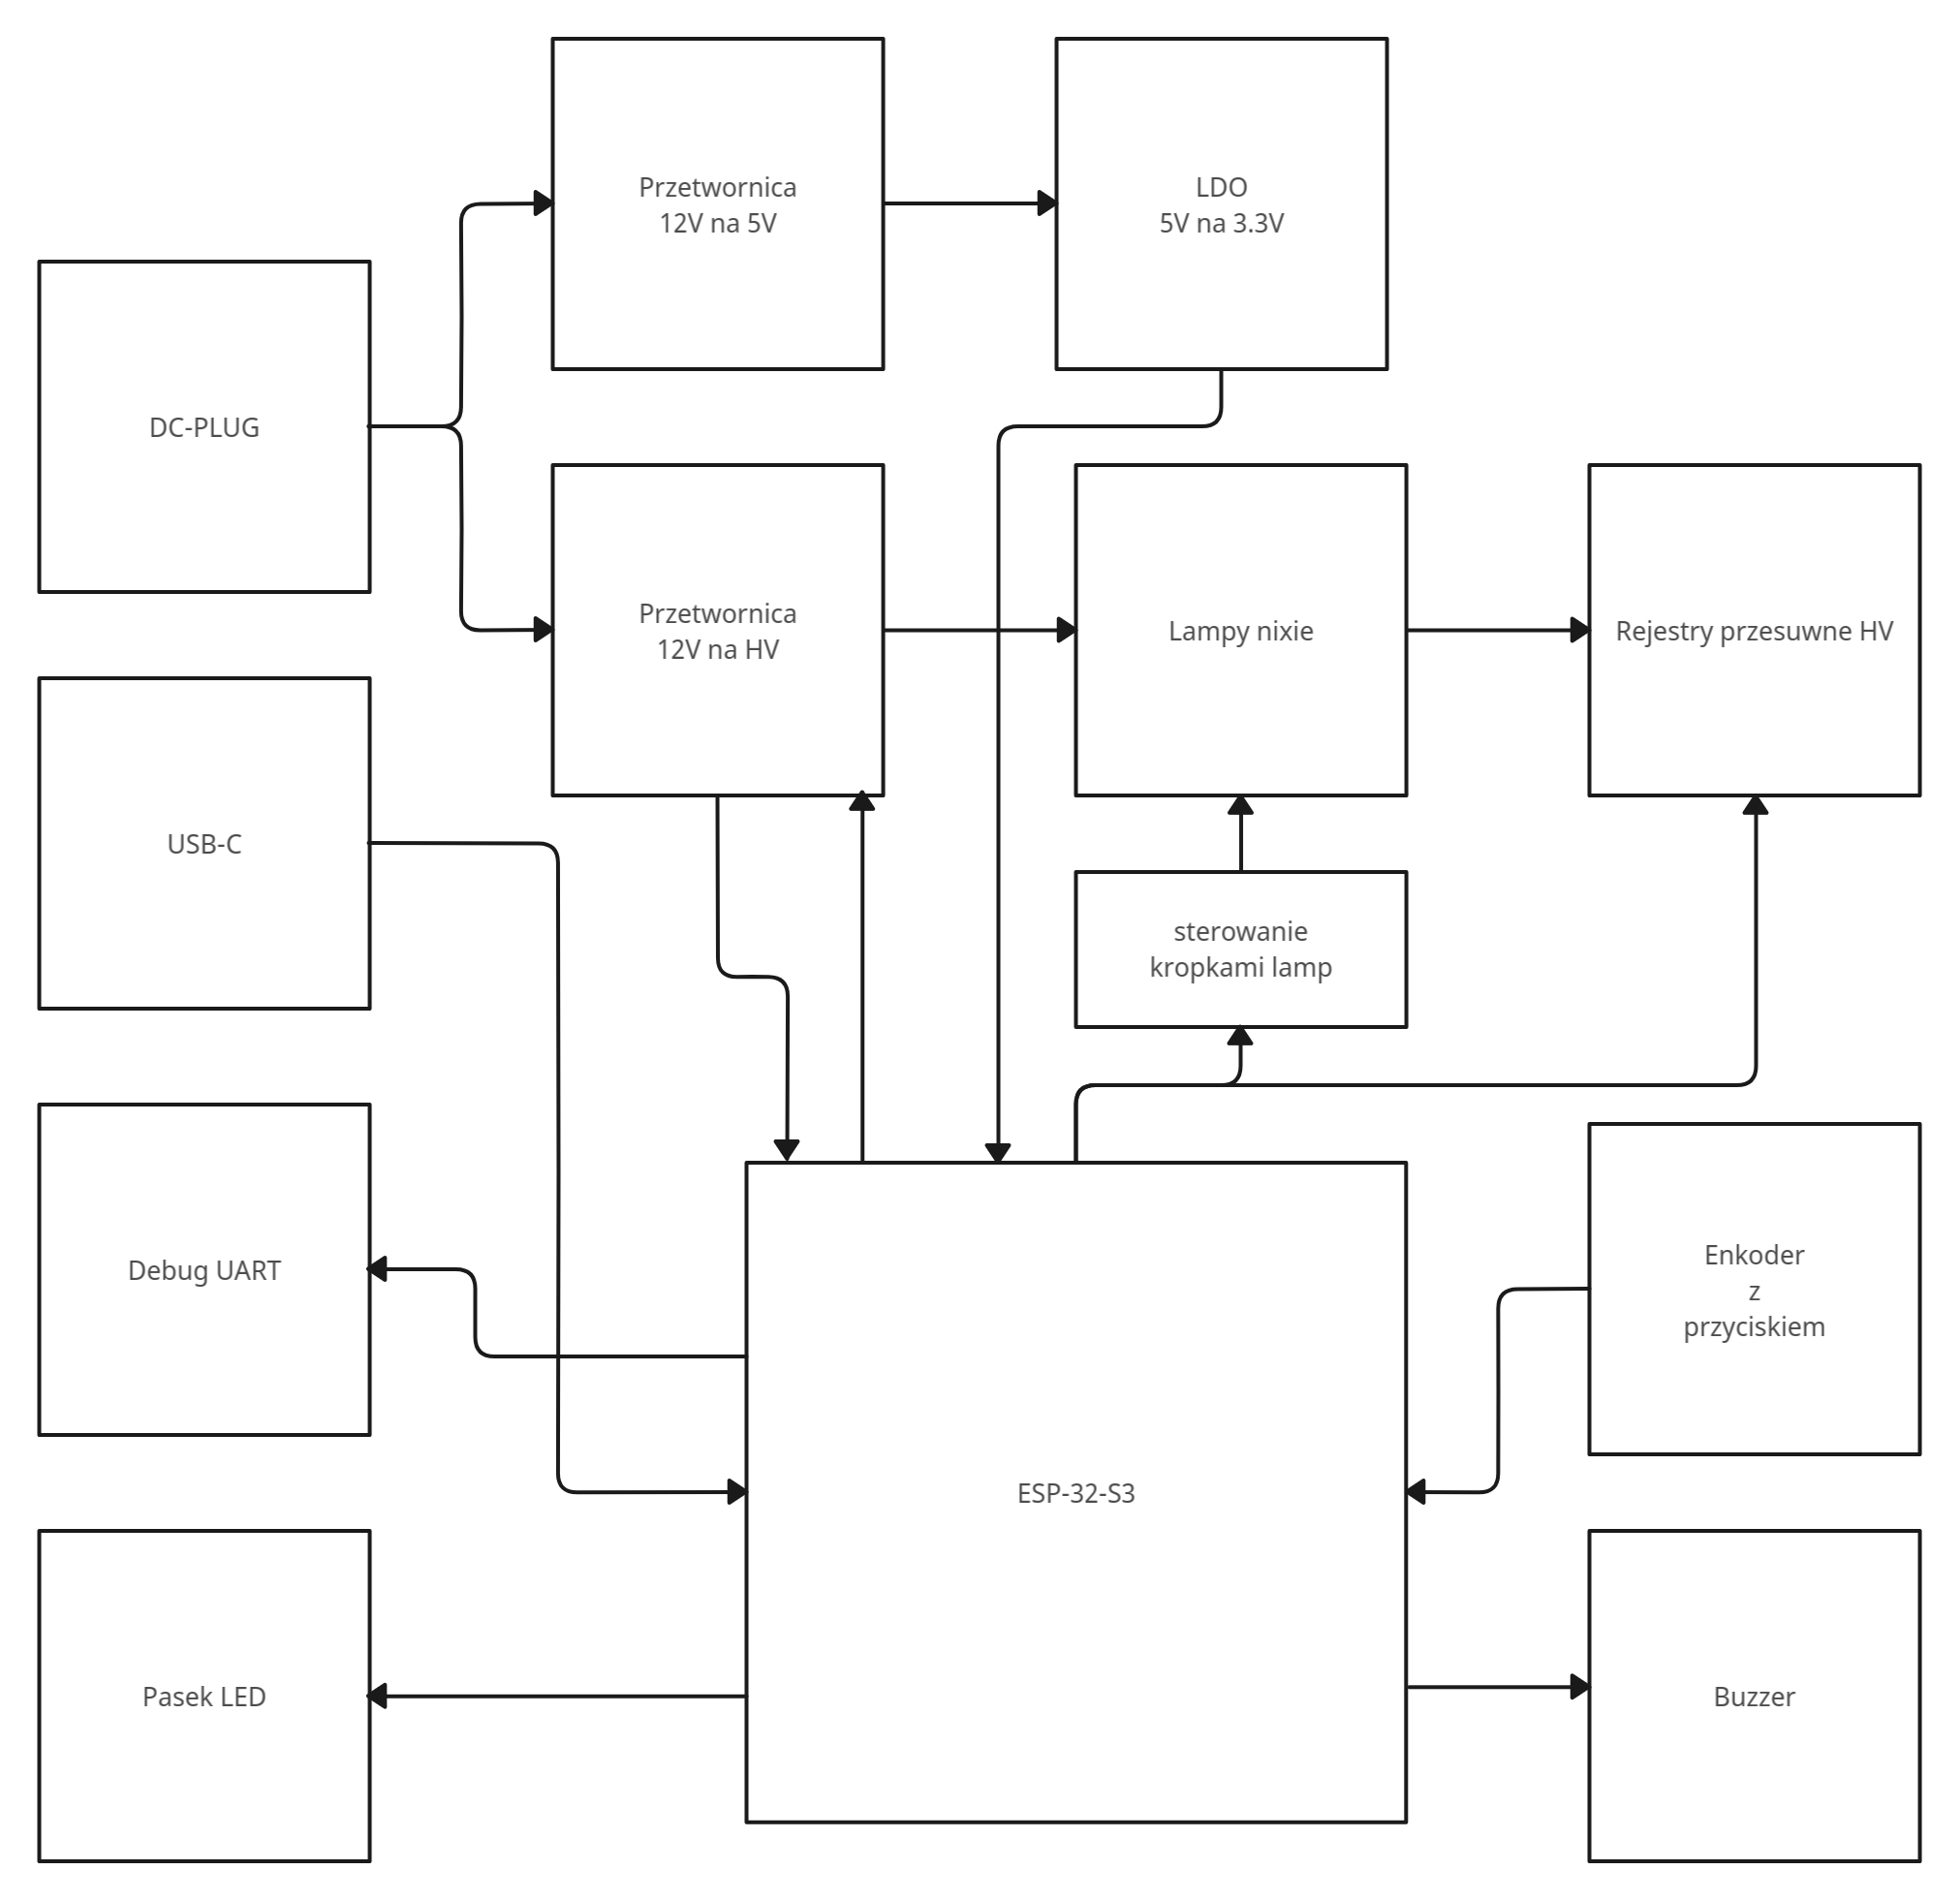
\includegraphics[width=1\textwidth]{schemat_blokowy.jpg}
    \caption{Schemat blokowy układu}
    \label{fig:schemat_blokowy}
\end{figure}

% \subsection{Dobór głośnika}
% Jako głośnik do budzika wybrano głośnik piezoelektryczny (buzzer) bez generatora. Wybór był podyktowany 
% małym rozmiarem, ponieważ wymaganiem jest by budzik był jak najmniejszy, a także niską ceną oraz prostotą w obsłudze.
% Buzzer bez generatora pozwala na generowanie dźwięku za pomocą prostego sygnału prostokątnego,
% co jest bardzo proste do zaimplementowania,, istnieje wiele bibliotek do generowania dźwięku na mikrokontrolerze.

\end{document}
